\let\lesson\undefined
\newcommand{\lesson}{\phantomlesson{Bài 1+2.}}


\setcounter{section}{2}
\section{Bài tập trắc nghiệm}
\begin{enumerate}[label=\bfseries Câu \arabic*:,leftmargin=1.5cm]
	\item \mkstar{1}\\
	{Đối tượng nghiên cứu của Vật lí là gì?
		\begin{mcq}
			\item Các dạng vận động và tương tác của vật chất.
			\item Quy luật tương tác của các dạng năng lượng.
			\item Các dạng vận động của vật chất và năng lượng.
			\item Quy luật vận động, phát triển của sự vật - hiện tượng.
		\end{mcq}
}
\hideall{
\textbf{Đáp án: C.}
}

\item \mkstar{1}\\
{Lĩnh vực nghiên cứu nào sau đây là của Vật lí?
	\begin{mcq}
		\item Nghiên cứu về sự thay đổi của các chất khi kết hợp với nhau.
		\item Nghiên cứu sự phát triển của vi khuẩn.
		\item Nghiên cứu về sự hình thành và phát triển của các tầng lớp, giai cấp trong xã hội.
		\item Nghiên cứu về các dạng chuyển động và các dạng năng lượng khác nhau.
	\end{mcq}

}
\hideall{
\textbf{Đáp án: D.}
}

\item \mkstar{1}\\
{Cách sắp xếp nào sau đây trong 5 bước của phương pháp thực nghiệm là đúng?
	\begin{mcq}
		\item Xác định vấn đề cần nghiên cứu, dự đoán, quan sát, thí nghiệm, kết luận.
		\item Quan sát, xác định vấn đề cần nghiên cứu, thí nghiệm, dự đoán, kết luận.
		\item Xác định vấn đề cần nghiên cứu, quan sát, dự đoán, thí nghiệm, kết luận.
		\item Thí nghiệm, xác định vấn đề cần nghiên cứu, dự đoán, quan sát, kết luận.
	\end{mcq}
}
\hideall{
\textbf{Đáp án: C.}
}


\item \mkstar{2}\\
{Thành tựu nghiên cứu nào sau đây của Vật lí được coi là có vai trò quan trọng trong việc mở đầu cho cuộc cách mạng công nghệ lần thứ nhất?
	\begin{mcq}
		\item Nghiên cứu về lực vạn vật hấp dẫn.
		\item Nghiên cứu về nhiệt động lực học.
		\item Nghiên cứu về cảm ứng điện từ.
		\item Nghiên cứu về thuyết tương đối.
	\end{mcq}
}
\hideall{
\textbf{Đáp án: B.}
}


\item \mkstar{2}\\
{Trong các hoạt động dưới đây, những hoạt động nào tuân thủ nguyên tắc an toàn khi sử dụng điện?
	\begin{mcq}
		\item Bọc kĩ các dây dẫn điện bằng vật liệu cách điện.
		\item Kiểm tra mạch có điện bằng bút thử điện.
		\item Sửa chữa điện khi chưa ngắt nguồn điện.
		\item Chạm tay trực tiếp vào ổ điện, dây điện trần hoặc dây dẫn điện bị hở.
		\item Thường xuyên kiểm tra tình trạng hệ thống đường điện và các đồ dùng điện.
		\item Đến gần nhưng không tiếp xúc với các máy biến thế và lưới điện cao áp.
	\end{mcq}
}
\hideall{
\textbf{Đáp án: A, B, E.}
}

\item \mkstar{2}\\
{Trong các hoạt động dưới đây, những hoạt động nào tuân thủ nguyên tắc an toàn khi làm việc với các nguồn phóng xạ?
	\begin{mcq}
		\item Sử dụng phương tiện phòng hộ cá nhân như quần áo phòng hộ, mũ, găng tay, áo chì, \dots
		\item Ăn uống, trang điểm trong phòng làm việc có chứa chất phóng xạ.
		\item Tẩy xạ khi bị nhiễm bẩn phóng xạ theo quy định.
		\item Đổ rác thải phóng xạ tại các khu tập trung rác thải sinh hoạt.
		\item Kiểm tra sức khoẻ định kì.
	\end{mcq}
}
\hideall{
\textbf{Đáp án: A, C, E.}
}
\end{enumerate}
\section{Bài tập tự luận}
\setcounter{section}{0}

\begin{enumerate}[label=\bfseries Câu \arabic*:,leftmargin=1.5cm]
	\item \mkstar{2}
	
	
	{ 
		
		Quan sát thiết bị thí nghiệm về nhiệt học và trình bày đặc điểm của các dụng cụ thí nghiệm trên. Những điều cần chú ý để đảm bảo an toàn khi tiến hành thí nghiệm với các dụng cụ này là gì?
		\begin{center}
			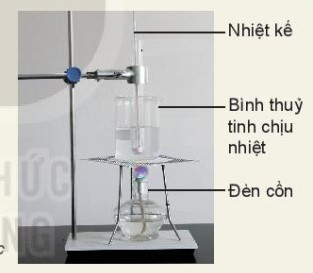
\includegraphics[scale=0.6]{../figs/VN10-2022-PH-TP003-3.jpg}
		\end{center}
	}
	
	\hideall
	{
		- Nhiệt kế: dùng để đo nhiệt độ của nước, hoạt động dựa trên cơ sở dãn nở vì nhiệt của các chất như: thủy ngân, rượu, ... được làm bằng thủy tinh dễ vỡ $\Rightarrow$ Khi tiến hành thí nghiệm cần cẩn thận, không để làm rơi, vỡ do thủy ngân trong nhiệt kế là một chất rất độc hại.
		
		- Bình thủy tinh chịu nhiệt: có thể chịu được nhiệt độ rất cao $\Rightarrow$ không dùng tay cầm trực tiếp vào bình.
		
		- Đèn cồn: dùng để đun sôi nước. Được thiết kế gồm:
		
		+ 1 bầu đựng cồn bằng thủy tinh
		
		+ 1 sợi bấc thường được dệt bằng sợi bông
		
		+ 1 chiếc chụp đèn bằng thủy tinh hoặc kim loại.
		
		$\Rightarrow$ \textbf{Lưu ý:}
		
		+ Không nên kéo sợi bấc quá dài
		
		+ Không trực tiếp thổi tắt ngọn lửa đèn cồn vì sẽ làm ngọn lửa cháy dữ dội hơn. Cách tốt nhất để tắt đèn là đậy nắp đèn cồn lại.
		
	}
	\item \mkstar{2}
	
	
	{
		Quan sát thiết bị thí nghiệm về quang học và trình bày đặc điểm của các dụng cụ thí nghiệm trên. Những điều cần chú ý để đảm bảo an toàn khi tiến hành thí nghiệm với các dụng cụ này là gì?
		
		\begin{center}
			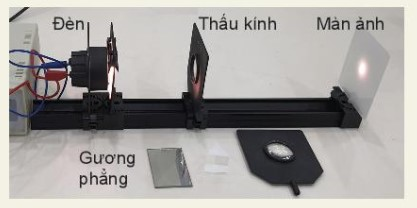
\includegraphics[scale=0.6]{../figs/VN10-2022-PH-TP003-4.jpg}
		\end{center}
	}
	
	\hideall
	{	
		- Đèn chiếu sáng: có kính tụ quang để tạo chùm tia song song, vỏ bằng nhôm hợp kim, có khe cài bản chắn sáng, có các vít điều chỉnh đèn. $\Rightarrow$ Tránh rơi, vỡ; để nơi khô thoáng.
		
		- Thấu kính: bằng thủy tinh, được lắp trong khung nhựa, gắn trên trụ nhôm $\Rightarrow$ Mỏng, dễ vỡ cần để trên cao, cất gọn gàng khi sử dụng xong.
		
		- Màn ảnh: có màu trắng mờ, gắn trên trụ nhôm $\Rightarrow$ Để nơi khô thoáng, tránh bụi bẩn.
		
		- Gương phẳng: bằng thủy tinh, dễ vỡ, sắc, nhọn $\Rightarrow$ Khi sử dụng cần cẩn thẩn, tránh va chạm mạnh hoặc rơi vỡ.
		
	}
	\item \mkstar{2}
	
	
	{
		Hãy quan sát một số hình ảnh về thao tác sử dụng các thiết bị thí nghiệm trong hình và dự đoán xem có những nguy cơ nào có thể gây nguy hiểm trong phòng thực hành vật lí.
		
		\begin{center}
			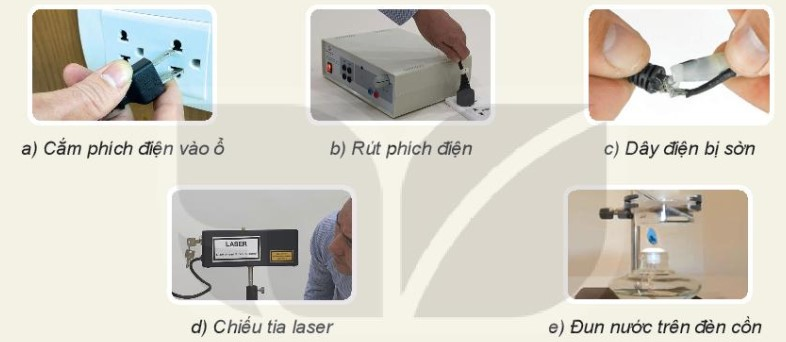
\includegraphics[scale=0.6]{../figs/VN10-2022-PH-TP003-5.jpg}
		\end{center}
	}
	
	\hideall
	{	
		\textbf{Nguy cơ có thể gây nguy hiểm}
		\begin{enumerate}[label=\alph*)]
			\item Cắm phích điện vào ổ: tay chạm vào phần kim loại dẫn điện ở phích điện $\Rightarrow$ bị giật.
			
			\item Rút phích điện: cầm vào phần dây điện, cách xa phích điện $\Rightarrow$ có thể làm dây điện bị đứt.
			
			\item Dây điện bị sờn: cầm tay trần vào dây điện mà không có đồ bảo hộ $\Rightarrow$ rất dễ bị giật điện.
			
			\item Chiếu tia laser: mắt nhìn trực tiếp vào tia laser gây nguy hiểm cho mắt.
			
			\item Đun nước trên đèn cồn: kẹp cốc thủy tinh quá gần với đèn cồn, bên dưới cốc không có lưới kim loại để phân tán nhiệt lượng (cốc sẽ dãn nở không đều) $\Rightarrow$ hư hỏng thiết bị thí nghiệm.
		\end{enumerate}
		
	}


	\item \mkstar{2}


{
	Hãy quan sát một số hình ảnh về thí nghiệm trong hình và dự đoán có những nguy cơ cháy nổ nào có thể xảy ra trong phòng thực hành.
	\begin{center}
		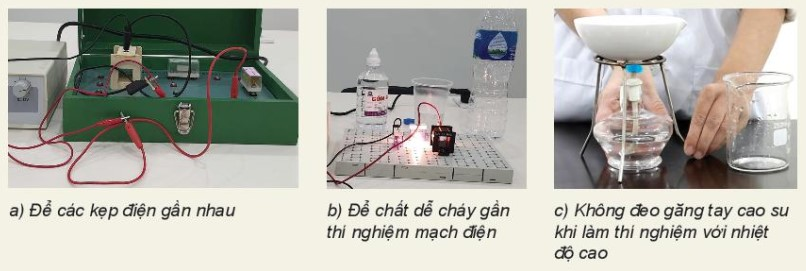
\includegraphics[scale=0.6]{../figs/VN10-2022-PH-TP003-7.jpg}
	\end{center}
}

\hideall
{	
	\begin{enumerate}[label=\alph*)]
		\item Để các kẹp điện gần nhau: có thể gây ra chập điện.
		\item Để chất dễ cháy gần mạch điện: nguy cơ cháy nổ.
		\item Không đeo găng tay cao su khi làm thí nghiệm với nhiệt độ cao, chạm tay trực tiếp vào đế kim loại khi đang đun: có thể bỏng.
	\end{enumerate}
}

	\item \mkstar{2}
	
	
	{
		Sử dụng động cơ điện có những ưu điểm vượt trội nào so với sử dụng máy hơi nước?
	}
	
	\hideall
	{	\begin{itemize}
			\item Ít tiêu tốn nhiên liệu vì hiệu suất chuyển hoá năng lượng cao.
			\item Hoạt động mạnh mẽ, tiết kiệm được thời gian vì động cơ điện có công suất lớn hơn nhiều so với động cơ hơi nước.
			\item Ít gây ô nhiễm môi trường do không phát thải khí thải thông qua quá trình đốt nhiên liệu.
		\end{itemize}
	}
	
	\item \mkstar{2}\\
	{Khí chiếu ánh sáng đến gương, ta quan sát thấy ánh sáng bị gương hắt trở lại môi trường cũ. Thực hiện những khảo sát chi tiết, ta có thể rút ra kết luận về nội dung định luật phản xạ ánh sáng như sau:
		\begin{itemize}
			\item Khi ánh sáng bị phản xạ, tia phản xạ sẽ nằm trong mặt phẳng chứa tia sáng tới và pháp tuyến của gương tại điểm tới.
			\item Góc phản xạ sẽ bằng góc tới.
		\end{itemize}
	Hãy xác định đối tượng cần nghiên cứu và phương pháp nghiên cứu trong khảo sát trên.
}
\hideall{
\begin{itemize}
	\item Đối tượng nghiên cứu: Sự truyền ánh sáng khi đến mặt gương.
	\item Phương pháp nghiên cứu: Phương pháp thực nghiệm.
\end{itemize}
}
	
	\item \mkstar{3}\\
	{Nhiều nhận định cho rằng: "Khoa học công nghệ ngày càng phát triển, bên cạnh việc chất lượng cuộc sống con người ngày càng được nâng cao thì con người cũng ngày càng đối diện với nhiều nguy hiểm". Em có ý kiến như thế nào về nhận định này? Bằng những hiểu biết Vật lí của mình, em hãy nếu các dẫn chứng cụ thể.
	
}
\hideall{
Học sinh đưa ra câu trả lời theo nhận định cá nhân:
\begin{itemize}
	\item Chất lượng cuộc sống con người ngày càng được nâng lên: nhiều thiết bị chăm sóc sức khoẻ, làm đẹp tại nhà; các thiết bị điện tự động hoặc điều khiển từ xa; vật dụng hiện đại trong nhà như bếp điện, nồi điện, máy hút bụi, \dots giúp cuộc sống con người tiện nghi hơn.
	\item Các nguy hiểm có thể có: rủi ro về điện như giật, cháy nổ, \dots; rủi ro phóng xạ từ các nhà máy điện hạt nhân; nguy cơ chiến tranh hạt nhân; \dots
\end{itemize}
}
	
	\item \mkstar{3}\\
	{Cho các biển báo như hình \ref{fig:2P-1}, hãy sắp xếp các biển này theo từng loại (biển báo cấm, biển báo nguy hiểm, biển thông báo) và cho biết ý nghĩa của từng biển báo.
		\begin{center}
			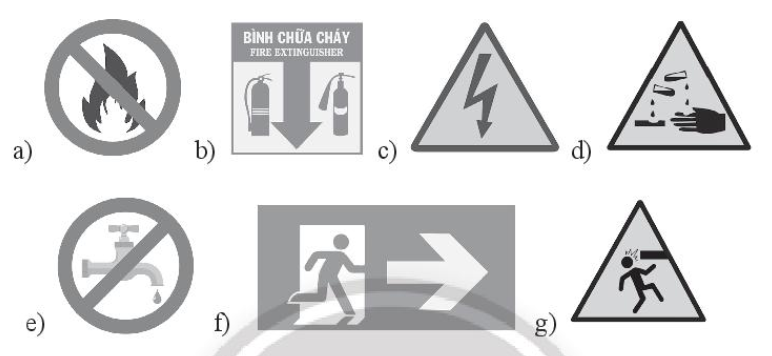
\includegraphics[width=0.6\linewidth]{../figs/VN10-2022-PH-TP002-P-1}
			\captionof{figure}{Một số biển báo}
			\label{fig:2P-1}
		\end{center}

}
\hideall{
\begin{itemize}
	\item Biển báo cấm: a (biển báo cấm lửa), e (biển báo cấm sử dụng nước).
	\item Biển báo nguy hiểm: c (biển cảnh báo nguy hiểm có điện), d (biển cảnh báo hoá chất ăn mòn), g (biển cảnh báo va chạm đầu).
	\item Biển thông báo: b (biển thông báo vị trí bình chữa cháy), f (biển thông báo lỗi thoát hiểm).
\end{itemize}
}

\item \mkstar{4}\\
{Ở những nơi nhiệt độ thấp (dưới $\SI{0}{\degree C}$), người ta nhận thấy rằng khi vung một lượng nước nhất định ra không khí thì nước nóng sẽ nhanh đông đặc hơn so với nước lạnh (Hình \ref{fig:2P-3}). Em hãy xây dựng tiến trình tìm hiểu hiện tượng trên, mô tả cụ thể các bước cần thực hiện, sau đó thực hiện tiến trình vừa xây dựng tại nhà và lưu lại kết quả thực hiện.\\
	\textit{Lưu ý: Chỉ nên sử dụng nước có nhiệt độ dưới $\SI{40}{\degree C}$ để đảm bảo an toàn trong quá trình thực hiện.}
	\begin{center}
		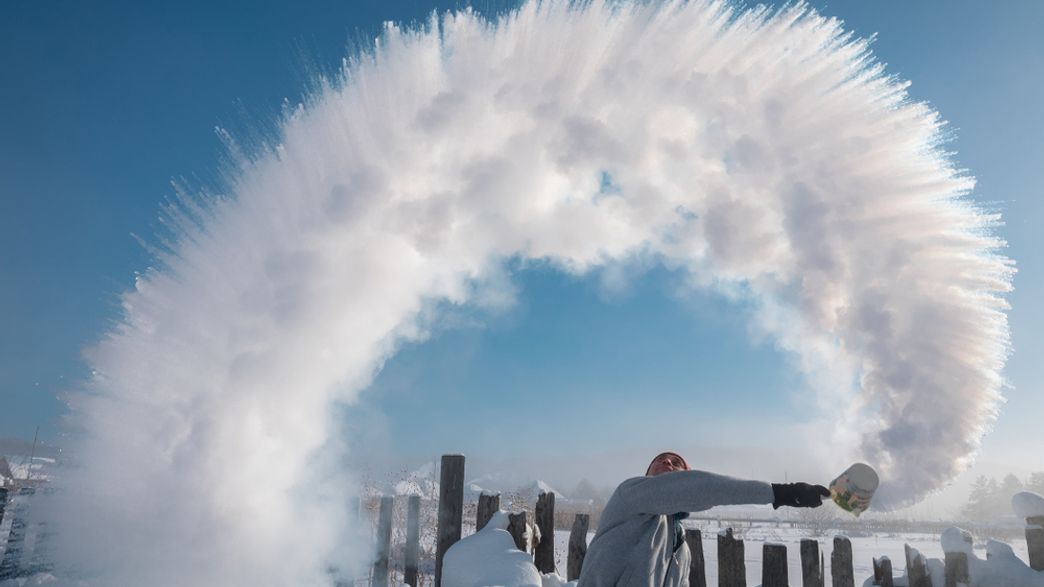
\includegraphics[width=0.3\linewidth]{../figs/VN10-2022-PH-TP002-P-3}
		\captionof{figure}{Nước nóng bị đông đặc ngay sau khi được vung ra ở nơi có nhiệt độ thấp.}
		\label{fig:2P-3}
	\end{center}
}
\hideall{
\textit{Tiến trình gợi ý:}\\
\begin{enumerate}[label=\arabic*.]
	\item Quan sát hiện tượng, các định đối tượng nghiên cứu: Nước nóng sẽ nhanh đông đặc hơn so với nước lạnh. Đối tượng nghiên cứu: Sự ảnh hưởng của nhiệt độ ban đầu đến thời gian đông đặc của nước.
	\item Giả thuyết đặt ra: Nước nóng đông đặc nhanh hơn nước lạnh.
	\item Lập phương án thực nghiệm: Khảo sát thời gian đông đặc của hai cốc nước có nhiệt độ khác nhau khi cho vào ngăn đông của tủ lạnh.
	\item Tiến hành thí nghiệm: Pha hai cốc nước (cùng thể tích) có nhiệt độ $\SI{5}{\degree C}$ và $\SI{35}{\degree C}$. Đặt hai cốc nước vào ngăn đông của tủ lạnh. Quan sát trạng thái đông đặc của hai cốc nước sau mỗi một giờ. Thu thập, xử lí và phân tích dữ liệu thực nghiệm.
	\item Rút ra kết luận.
\end{enumerate}
}
\end{enumerate}